\documentclass{specification}
\usepackage[backend=bibtex]{biblatex}
\usepackage{dsfont}
\usepackage{graphicx}
\usepackage{epstopdf}
\bibliography{bibliography}


\title{Outline of ``Automated Protein Function Description for Novel Class Discovery''}
\author{Meet Barot}

\begin{document}

\maketitle

\section{Abstract}
High-throughput sequencing technologies have allowed us to amass millions of protein sequences from organisms throughout the tree of life.
Protein function prediction, as it is framed in the case of Gene Ontology term prediction, is a multilabel problem with a hierarchical label space.
However, this framing is limiting as it does not provide guiding principles for discovering completely novel functions.
Clustering-based approaches are not able to give much information about the new functional categories that they predict; they can only predict that a protein may belong to a category that has not been studied.
In this work we propose a neural machine translation model in order to generate descriptions of protein functions in natural language.
We provide quantitative results of our model in the zero-shot classification setting, scoring functional descriptions that the model has not seen before, as well as function descriptions for qualitative evaluation.

\section{Introduction}

    \subsection{Motivation}
    Why make a model that describes the common functions of a set of proteins in natural language?
    \begin{enumerate}
        \item We want to be able to predict the functions of proteins, but we are limited by the amount of data that we have in both the amount of well characterized proteins and also the variety of known functions.
        \item Even the best supervised approaches can only take us to the point where we can annotate proteins that have functions that have been seen before.
        \item Explicitly ontology-based zero-shot approaches such as DeepGOZero \cite{DeepGOZero} do not allow for actual description of a new function that is discovered.
The only information that is gained is that the protein has a new function that has some specified ontological relation to currently known functions.
However, this may not sufficiently describe the new function, and it also excludes possible functions that do not directly relate to known functions.
    \end{enumerate}
    In order to discover new categories of protein function, with some amount of information to actually design experiments to test for them, we need a model that generates functional descriptions.

\section{Related Work}
\subsection{Protein Function Prediction}
Many methods have been proposed for protein function prediction, though most do not consider the problem of discovering novel functions.
Instead, the task is generally framed as a supervised multilabel problem where the predicted labels are all assumed to have some example in the training set.
Yet most unlabeled proteins, especially in understudied organisms, are likely to perform functions that have not yet been characterized.
The supervised approach does not address this possibility, and so new methods must be proposed for function discovery.

Clustering-based approaches are not able to give much information about the new functional categories that they predict.
They can only predict that a protein may belong to a category that has not been studied.
One could compute average distances to clusters that contain known proteins, but beyond this, there is no testable hypothesis that the model can give about their function.

Zero-shot learning approaches attempt to address the unseen class problem as well, mostly by creating continuous embeddings of the labels and predicting a mapping from the input to real-valued vectors in that learned label space \cite{CLIP}.
Similar to clustering-based approaches, not much information about the unseen class is gained besides its distance from existing categories and its direction in the abstract label space.
DeepGOZero \cite{DeepGOZero} is a method that uses ontology axioms to predict for classes with no examples in the training set.
However, the classes that are able to be predicted must be defined with ontological relations to seen classes.
This constraint both restricts the possible novel functions that can be discovered and may not give sufficient information to design an experiment to test for the novel function.
Among the few zero-shot approaches proposed for function prediction, none are able to describe the novel functions discovered in natural language.

\subsection{Neural machine translation}

\section{Methods}
\begin{figure}
    \centering
    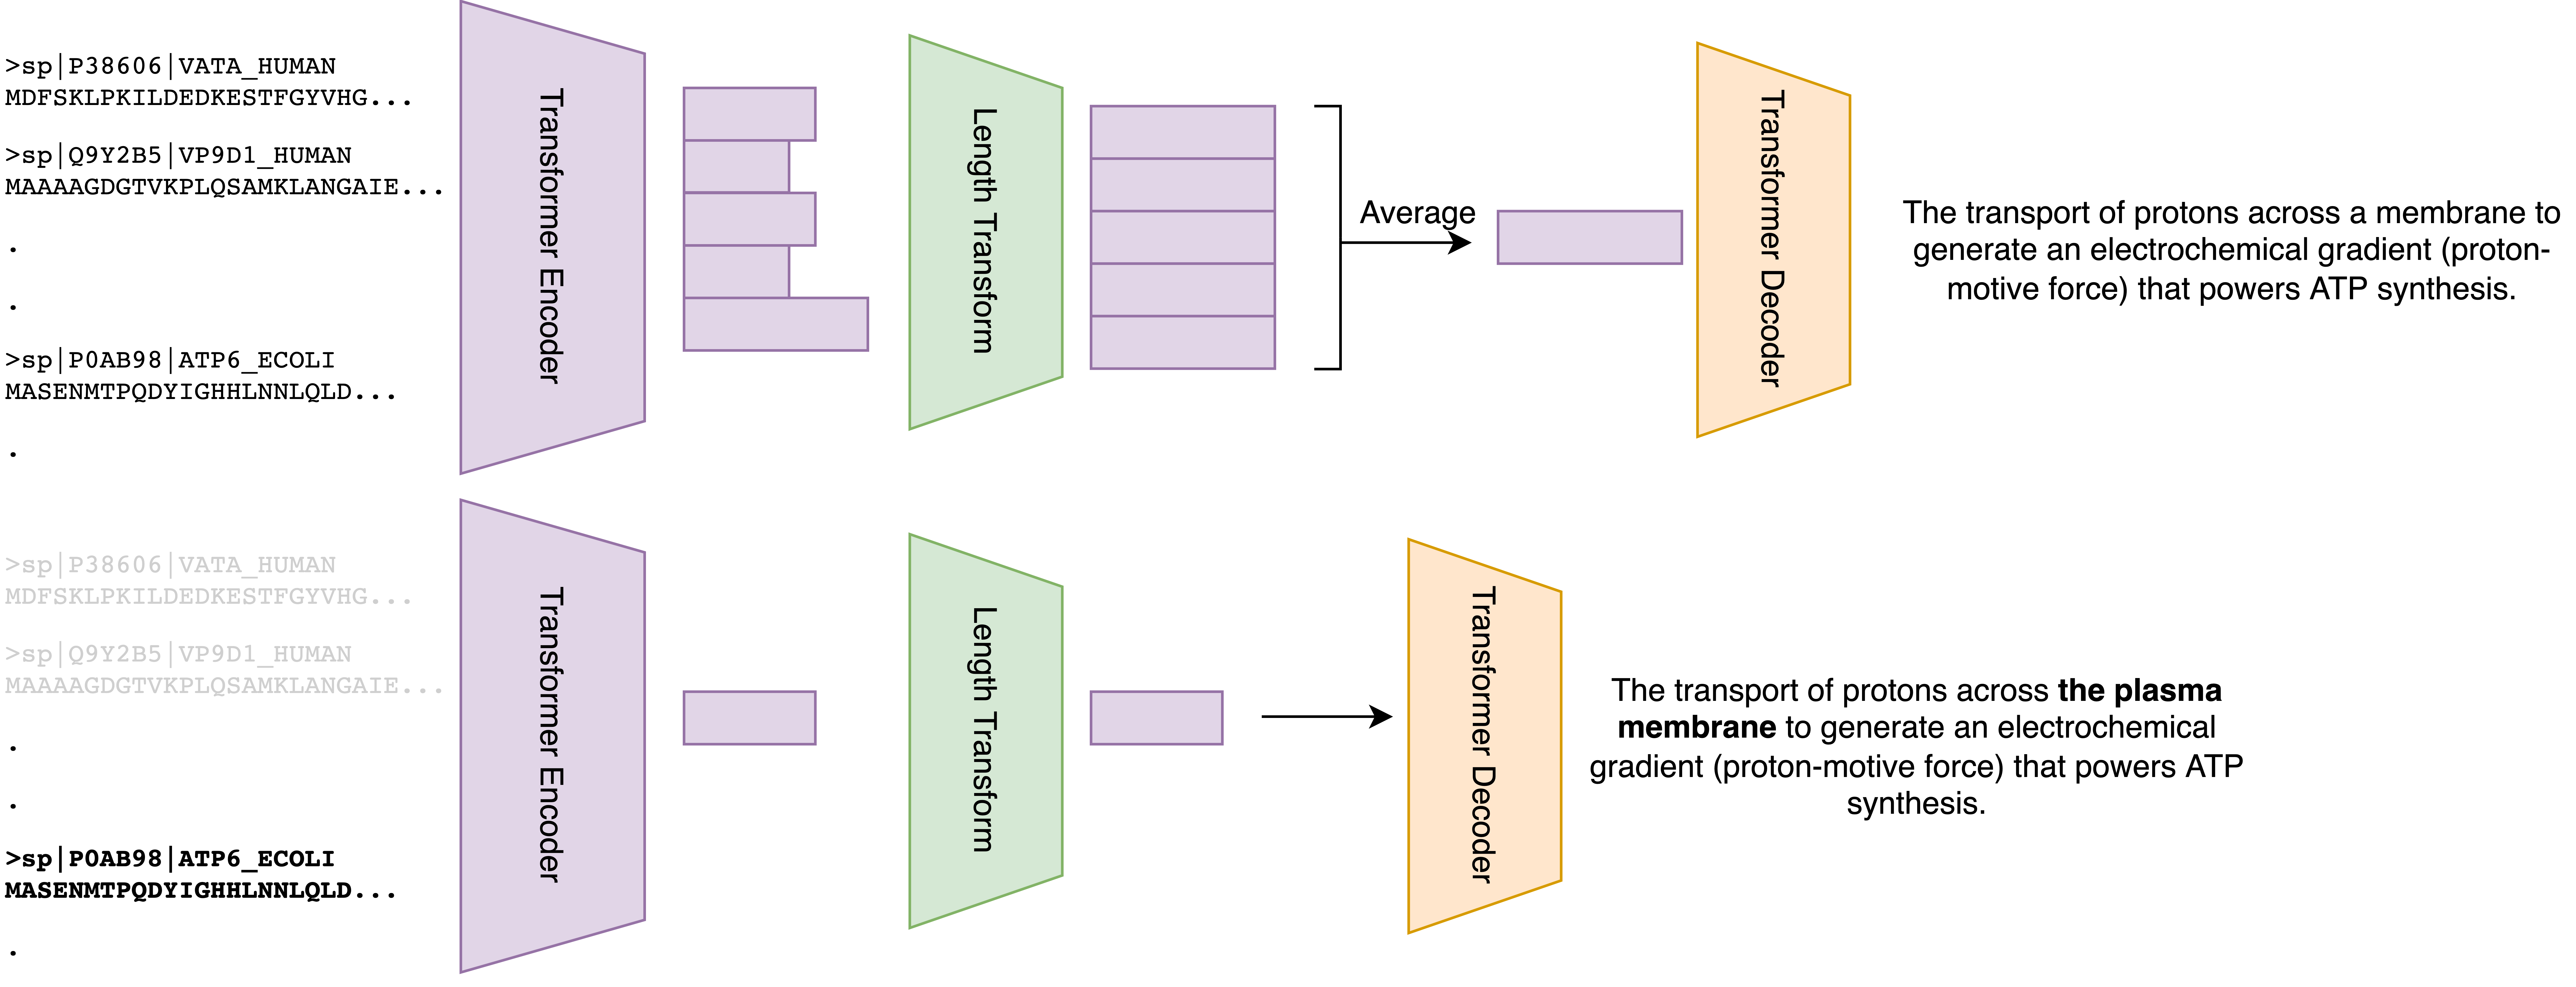
\includegraphics[width=0.9\linewidth]{prot2go.png}
    \caption{High-level diagram of the proposed transformer encoder-decoder model.
The model is trained to produce the most specific common function of the input protein sequences.}
    \label{overview}
\end{figure}
    \subsection{Transformer encoder-decoder model}
    We use a transformer encoder-decoder model \cite{vaswani2017} with a length transform \cite{Shu2019} to handle differing sequence lengths in order to average sequence features from the encoder.
    \subsection{Length transform}
    \subsection{Zero-shot Classification setting}
    \subsection{Generation (beam search)}
\section{Evaluation}
In this section, we define three metrics that can be computed using known functional descriptions in order to evaluate our models' learned probability distributions.

Generated descriptions are shown in the Results section for qualitative analysis.
Quantitative analysis of the generated descriptions requires data from human evaluators with expertise in protein function in order to determine the accuracy of generated descriptions.
A framework for performing that analysis with expert curators is explored in the Discussion section.
    \subsection{Metrics}
        \subsubsection{Attribute 1: Annotation correctness.}

        Given a sequence set for which the model is assigning scores to function descriptions, descriptions of GO terms that annotate the entire sequence set should be scored higher than terms that do not annotate the entire sequence set.

        Let $D_{S}$ be the GO term descriptions associated with sequence set S.

        \[P(d \in D_{S} | S) > P(d \notin D_{S} | S)\]

        A way to measure this attribute would be to calculate:
        \[\frac{1}{|D_{S}|*|D_{S}^{c}|}\sum_{d_i \in D_{S}, d_j \notin D_{S}} \mathds{1}(P(d_i | S) > P(d_j | S))\]
        where $D_{S}^{c}$ is the complement of $D_{S}$ and $\mathds{1}$ is the indicator function.

        \subsubsection{Attribute 2: Specificity preference.}

        Among terms that do annotate the whole set, the model should score child terms higher than their ancestor terms.
Let $A(d)$ denote the description of a direct parent of the GO term described by $d$.

        \[P(d \in D_{S}| S) > P(A(d) \in D_{S}| S)\]
        Note: any protein set that is annotated with $d$ would always be annotated with $A(d)$, $A(A((d))$ and so on.

        A way to measure this attribute would be to calculate:
        \[\frac{1}{|D_{S}|}\sum_{d_i \in D_{S}} \mathds{1}(P(d_i | S) > P(A(d_i) | S))\]

        \subsubsection{Attribute 3: Annotation robustness.}

        Any set of sequences that have the same exact set of GO descriptions in common should produce scores with the same rankings for those GO descriptions.

        Let $S_i$ and $S_j$ be different sequence sets such that $D_{S_i} = D_{S_j}$ and $S_i \neq S_j$, and let $R(X)$ be a ranking function that gives the ranks of entries in $X$, in descending order.

        \[R_{d}(P(d \in D_{S_i} | S_i)) = R_{d}(P(d \in D_{S_i} | S_j))\]

        A way to measure this attribute would be to calculate the average Spearman's rank correlation of the rankings for all sequence sets' correct descriptions.
Let $R_{S_i} = R(P(D_{S_i} | S_i))$:

        \[\frac{1}{N*(N-1)}\sum_{S_i, S_j} \frac{\textnormal{cov}(R_{S_i}, R_{S_j})}{\sigma_{R_{S_i}}\sigma_{R_{S_j}}}\]

        where $N$ is the total number of sequence sets that have the exact set of GO descriptions $D_{S_i}$.
In reality, this number may be too large to actually sum (especially if $|D_{S_i}|$ is small), so we approximate this measure by subsampling $n < N$ sequence sets to average over instead.
The sum is only calculated over non-identical pairs of sequence sets.

\section{Results}
\begin{enumerate}
    \item Plots of the models with the three metrics.
Training proteins with training GO terms, test proteins with training GO terms, and test proteins with test GO terms.
    \item Analysis of what differences the models have in terms of architecture or training, and how that relates to the difference in performances across the three measures.
    \item Table of randomly selected generated descriptions of protein sets that have GO terms not in the training set for each model.
    \item Perhaps some analysis of the model's performance with respect to point anomalies, contextual anomalies, group anomalies? Would likely need to create specific datasets for these tests
\end{enumerate}

\section{Discussion}
In this work, we have proposed a novel method to generate protein function descriptions in order to discover new protein functions.
We have demonstrated that our model can accurately rank unseen function descriptions for proteins not seen in the training set, and show promising results in generated function descriptions.
Below, we explore how we might further evaluate the method's generated descriptions using human expertise and curation.

\subsection{Future human-assisted evaluation of function discovery}
As our scoring metrics for evaluation are automated, they can be used for optimizing the architecture and other hyperparameters of the model (either manually or with some search method).
However, in the case of actual use on proteins that are not very well studied, it can be difficult to know whether a given description is accurate.
Human-assisted evaluation will be needed for the descriptions generated for a given set of novel proteins.
This feedback could be used to fine-tune the model to produce more accurate, fluid or generally desirable descriptions of proteins, as has been done for document summarization models \cite{finetuningWithHuman, learningToSummarize}.

One possible way of obtaining human feedback would be to ask an expert with knowledge of the Gene Ontology and familiarity with some families of proteins to choose between two descriptions for a given sequence set that is generated from a trained model.
Doing this over a large enough dataset would allow us to train a reward estimation model that can then be used to fine-tune the original trained model using reinforcement learning.
However, this would be expensive, as the task needs to be done by an expert.
Richer information, such as ranking the similarities to an existing GO term, or suggesting changes to particular portions of the description, could be used to increase performance even with a small number of examples with human feedback.

\printbibliography

\end{document}
